\appendix
\section{Event selection}\label{app:sel}

The seven requirements of Table~\ref{tab:sel} are applied in the order shown. The last one uses
the highest-$p_T$ $b$-tagged jet; the alternative of ordering the tagged jets by truth flavour is
discussed in Section~\ref{sec:sys}.

\begin{table}[htbp]
\centering
\caption{Selection requirements of the CMS all-hadronic $0\ell2b$ signal region, applied in the order shown. The last requirement defines the $b$ jet used in the transverse-mass cut; the treatment of that choice is discussed in Section~\ref{sec:sys}.}
\label{tab:sel}
\begin{tabular}{ll}
\toprule
Requirement & Value \\
\midrule
Lepton veto & no electron or muon with $p_T>10$~GeV and $|\eta|<2.4$ \\
Jets & at least three with $p_T>30$~GeV, $|\eta|<2.4$ \\
$b$-tagged jets & at least two \\
Missing transverse momentum & $p_T^{\rm miss}>250$~GeV \\
Leading-jet momentum fraction & $p_T(j_1)/H_T<0.5$ \\
Azimuthal separation & $\min\Delta\phi(j_{1,2},p_T^{\rm miss})>0.8$ \\
Transverse mass & $m_T^b>140$~GeV \\
\bottomrule
\end{tabular}
\end{table}

\noindent{\footnotesize Here $H_T$ is the scalar sum of the transverse momenta of the selected jets, and $m_T^b=\sqrt{2\,p_T^{b}p_T^{\rm miss}\left(1-\cos\Delta\phi_{b}\right)}$ with $b$ the highest-$p_T$ $b$-tagged jet among the selected jets, the definition used throughout the analysis.}

\section{Experimental input}\label{app:input}

The expected limits use the published post-fit background and data distributions of the CMS
all-hadronic $0\ell2b$ signal region, reproduced in Fig.~\ref{fig:cmsinput} from
Ref.~\cite{CMS}; the last bin contains the overflow and no aspect of the distributions has been
modified.

\begin{figure}[htbp]
\centering
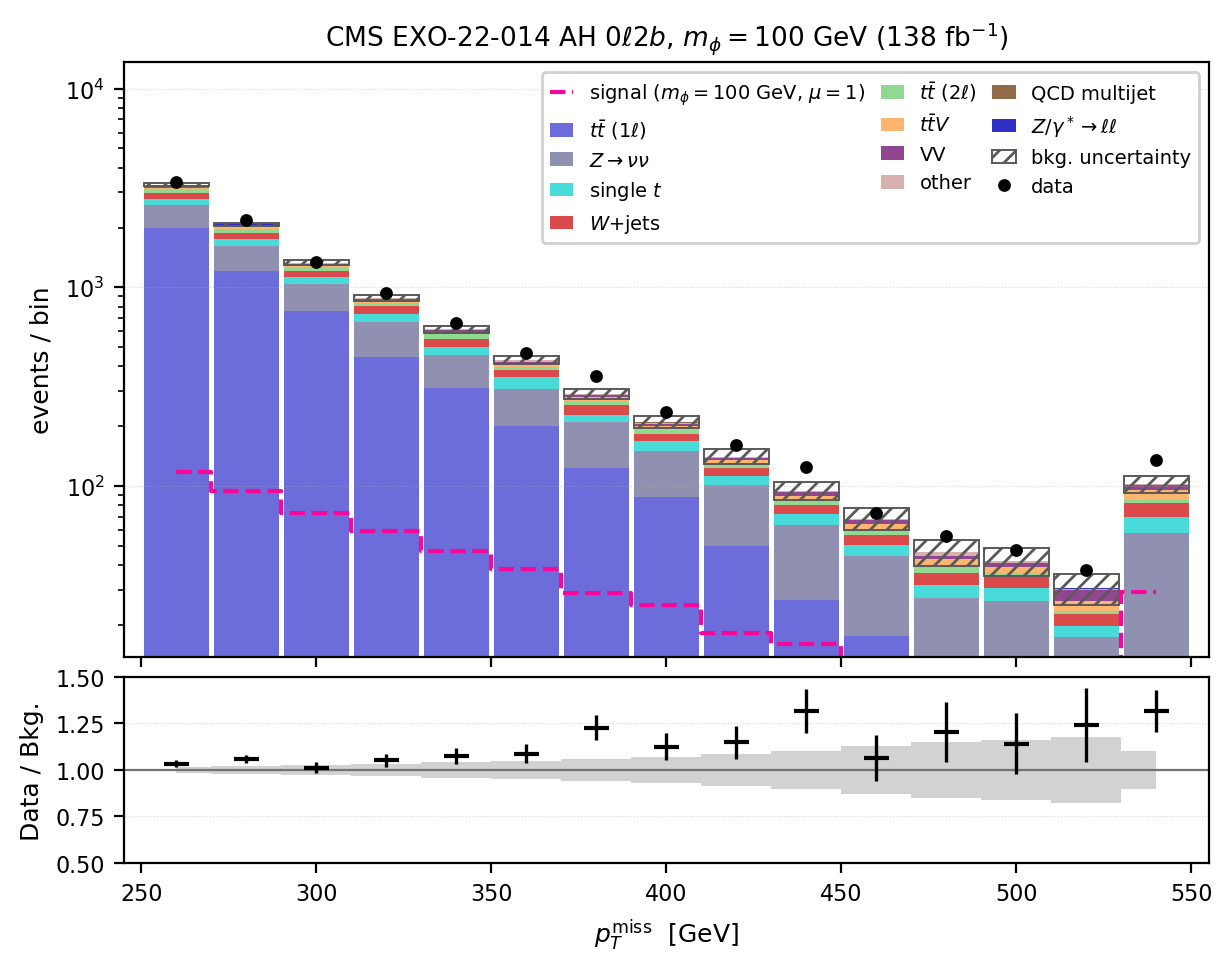
\includegraphics[width=0.64\textwidth]{figs/fig2_cms_inputs.png}
\caption{\textbf{CMS published figure (external input).} Post-fit $p_T^{\rm miss}$
distribution in the CMS all-hadronic $2b$ signal region, reproduced from Ref.~\cite{CMS}.
It is shown to document the background
and data inputs. The last bin contains the overflow events.}
\label{fig:cmsinput}
\end{figure}

\begin{table}[htbp]
\centering
\caption{Selection efficiency by mediator-mass column. The third column gives the minimum, median and maximum efficiency within the column, $\delta\varepsilon$ is the binomial uncertainty at the median point, quoted in percentage points, and the last column is the fraction of generated events that pass the $p_T^{\rm miss}>250$~GeV requirement, applied after the jet, $b$-tag and lepton requirements as listed in Table~\ref{tab:sel}. All 470 points are used.}
\label{tab:eff}
\begin{tabular}{crcccc}
\toprule
$M_V$ [GeV] & points & $\varepsilon$ [\%] (min / median / max) & $\delta\varepsilon$ [percentage points] & $p_T^{\rm miss}>250$ [\%] \\
\midrule
20 & 44 & 0.662 / 0.865 / 1.100 & 0.065 & 1.16 \\
30 & 44 & 0.950 / 1.120 / 1.255 & 0.074 & 1.49 \\
40 & 44 & 1.050 / 1.400 / 1.615 & 0.083 & 1.85 \\
50 & 44 & 1.475 / 1.647 / 1.815 & 0.090 & 2.24 \\
60 & 44 & 1.738 / 1.916 / 2.262 & 0.153 & 2.66 \\
70 & 44 & 2.035 / 2.282 / 2.565 & 0.106 & 3.05 \\
80 & 43 & 2.288 / 2.575 / 2.975 & 0.112 & 3.40 \\
90 & 38 & 2.565 / 2.813 / 3.080 & 0.117 & 3.82 \\
100 & 34 & 2.890 / 3.107 / 3.505 & 0.122 & 4.21 \\
120 & 27 & 3.540 / 3.810 / 4.115 & 0.135 & 5.12 \\
140 & 22 & 4.140 / 4.353 / 4.685 & 0.144 & 5.93 \\
160 & 17 & 4.825 / 5.010 / 5.595 & 0.154 & 6.80 \\
180 & 14 & 5.285 / 5.665 / 6.070 & 0.163 & 7.56 \\
200 & 11 & 5.930 / 6.240 / 6.585 & 0.171 & 8.43 \\
\bottomrule
\end{tabular}
\end{table}

